\documentclass[pdftex,paper=A4,DIV=calc,titlepage,12pt]{scrartcl}

%Global options
\usepackage[paper=a4paper,includefoot,includehead,left=20mm,right=20mm,top=20mm,bottom=20mm]{geometry}
\usepackage[pdftex]{graphicx}
%\usepackage[colorlinks=true,
	    %linkcolor=red,
	    %anchorcolor=black,
	    %citecolor=green,
	    %pagecolor=red,
	    %urlcolor=cyan
	    %]
	    %{hyperref}
\usepackage{nameref}

\usepackage{tikz}
\usetikzlibrary{calc,arrows,matrix,fit,positioning}

%Page header
\usepackage{fancyhdr}
\usepackage{fancyhdr} 
\pagestyle{fancyplain}
\headheight\baselineskip
\topmargin-0.75cm
\textheight47\baselineskip
\def\MakeUppercase#1{#1}
\makeatletter
\lhead[\fancyplain{}{\thepage}]
      {\fancyplain{}{\slshape Burrows-Wheeler-Transformation}} % <--- Titel eintragen
\rhead[\fancyplain{}{\slshape Uli Köhler	}]    % <--- Name eintragen
      {\fancyplain{}{\thepage}}
\cfoot[]{}
\makeatother


%Theorems
\usepackage{thmbox} %Boxed theorems

%Tables, Floats and figures
\usepackage{array}
\usepackage{float} %COnfigure figure floats to be boxed
  \floatstyle{boxed}
  \restylefloat{figure}

%Special formats
\usepackage{url}

%Citations and references
\usepackage{cite}
\usepackage{fancyref}
\usepackage{varioref}
%%\renewcommand{\reftextfaceafter}{auf der \reftextvario{gegenüberliegenden}{nächsten} Seite} 
%%\renewcommand{\reftextfacebefore}{auf der \reftextvario{gegenüberliegenden}{vorherigen} Seite} 
%%\renewcommand{\reftextafter}{auf der \reftextvario{nächsten}{folgenden} Seite} 
%%\renewcommand{\reftextbefore}{auf \reftextvario{der vorhergehenden}{der letzten} Seite} 
%%\renewcommand{\reftextcurrent}{auf \reftextvario{der aktuellen}{dieser} Seite}


%Typography, language and error corrections:
\usepackage[utf8x]{inputenc}
\usepackage[T1]{fontenc}
\usepackage{lmodern} %Latin modern = enhanced CM font
\usepackage{xspace} %Space enhancements
\usepackage[tracking=true,activate={true,nocompatibility}]{microtype} %PDFTeX typography enhancements
\usepackage{fixltx2e}
%Line spacing
\usepackage{setspace}

\usepackage{inconsolata}


%Header declarations
\pagestyle{headings}

%Create a new boxed type of theorems
\newtheorem[L]{boxedDefinition}{Definition}
\newtheorem{definition}{Definition}

\setcounter{secnumdepth}{3}
\setcounter{tocdepth}{3}

%Scriptsized, vertically and horizontally centered tabular column type
\newcolumntype{s}[1]{>{\scriptsize\centering\arraybackslash}m{#1}}


\title{3D-Tumorvisualisation}
\subtitle{Seminararbeit}
\author{Uli Köhler}
%\institute[EMG]{Ernst-Mach-Gymnasium Haar}
\date{9.~November 2010}

\newcommand{\footnoteremember}[2]{\footnote{#2}\newcounter{#1}\setcounter{#1}{\value{footnote}}}
\newcommand{\footnoterecall}[1]{\footnotemark[\value{#1}]}
%Utility to insert a newline after a paragraph declaration
\newcommand{\paranl}{$~~$\\}
\newcommand{\HRule}{\rule{\linewidth}{0.5mm}}
\sloppy
\begin{document}
\begin{titlepage}
\begin{center}
 \end{center}
\vspace{2cm}
\begin{center}
 \large\textsc{Seminar report}\\[5mm]
 {\Huge\centering\bfseries\selectfont Phylogenomic inference}\\[2cm]
\begin{center}
  Uli Köhler -- 2014-02-03
\end{center}
\vspace{2cm}
\end{center}
\tableofcontents
\end{titlepage}

\section{Introduction}
Since high-throughput sequencing is commercially available, computational biologist are facing an ever-increasing amount of genomic and proteomic data.

In order to leverage all this information for applications like in-silico drug target searching, advanced methods have been developed that use databases of known protein properties in order to infer properties of new proteins.

The most interesting property of any protein is its function -- if the function would be known for any protein in the proteome, it would be relatively easy to derive potential drug targets from this information.

One of the most important concepts in this area of bioinformatics is homology-based function prediction: Proteins of high similarity have a high probability of having a similar or identical function that has possibly been conserved in the evolutional history of the organism.

However, in order to assess protein function with high significance, the analysis has to use information from all available sources in order to eliminate as many sources of error as possible.

This report will summarize Phylogenomics, a methodology to augment prediction quality by using phylogenetics in order to differentiate orthologs and paralogs, with the former having a higher probability of conserving their function during evolution.

\section{Issues of non-phylogenomic function prediction}\label{sec:nonphylo-issues}

Classical function prediction methods are often built on the comparison of protein features like tertiary structure.

This concept is based on the assumption that if structural elements like domains are conserved in a protein family, there is a significant probability that the element is critical for the family-specific function.

For most proteins that are known today however, the tertiary structure is not known -- the PDB database currently contains \textasciitilde$90000$\footnote{2014-02-03} structures, whereas  \textasciitilde$5.1\times10^6$ UniProt/TrEMBL\footnote{2014-02-03, combined} sequences.

This huge discrepancy is mainly based on the expensiveness of structural assessment methods like X-ray crystallography that not only require a specialized laboratory, but also -- for each individual experiment -- expert knowledge to crystallize the protein and assess the X-ray crystallogram. To date, only few advances have been made in automation of those methods (a summary is provided at \cite{groves2007recent}) and most of them require a high-quality X-ray beam only available in particle accelerators like Synchrotrons which are not available to most laboratories.

In the future, this discrepancy is expected to increase even more, because commercially available sequencers drop in price rapidly and allow semi-automatic sequencing with a speed of several Gigabases per day. Besides these devices yielding a large amount of predicted proteins, recent advances have been made in an area called \textit{shotgun proteomics} that use shotgun sequencing methods well-known from genomic sequencing methodologies in order to sequence proteoms directly. As described in \cite{wu2002shotgun}, these methods are available since more than ten years and will.

Therefore, in order to cope with the massive amount of sequence-only proteins, computational biology tries to infer protein functions from sequence and relations to known proteins.

\paragraph{Systematic errors of non-phylogenomic prediction}\label{p:syserrors}
While those methods yield high-quality predictions for a large number of proteins, there are several systematic errors outlined in \cite{brown2006functional}:

\begin{itemize}
 \item \textit{Gene duplication} is not taken into account, yielding a predicted orthology, while the proteins would have to be considered paralog
 \item \textit{Domain shuffling} events that cause highly similar sequences to have different protein functions due to a largely different structure
 \item \textit{Evolutionary distance} is not used to augment the prediction, therefore the chance of homolog proteins having the same function in distantly-related species is overrated.
\end{itemize}

\section{Phylogenomic methodology}

Phylogenomics attempts to minimize the influence of aforementioned errors by improving homology metrics using phylogenetic information that provides knowledge about the evolutionary history of the protein in question.

The core concept of phylogenomics is the differentiation of homologs into orthologs and paralogs.

Orthologs have a higher probability of conserving function over evolution, whereas two proteins identified as paralog usually have different functions.

If sufficient data is available to build a phylogenetic tree\footnote{Generally, the tree can be deduced from a sequence set alone, however this approach w ould introduce too much noise}, phylogenomic algorithms classify branching points in the tree as either duplication  or speciation, with the former yielding paralog proteins whereas the latter yields orthologs (see \cite{eisen2003phylogenomics}). This process is called \textit{tree reconciliation}

A conceptual example of what is classified is visualized in figure \vref{fig:dupsec}.

\begin{figure}[ht!]
\centering
\caption{Concept of Phylogenomics: Differentiating orthologs and paralogs}
\label{fig:dupsec}
\begin{tikzpicture}
\tikzset{
  protein/.style = {block, align=center, text centered,fill=orange,
		    draw, rectangle, rounded corners},
  ancestor/.style = {block,minimum size=0cm},
  connection/.style = {thick,draw,arrowhead=4mm, line width=2pt}
};
%Protein nodes
\node [protein] (proteinA) {A};
\node [protein, right=2cm of proteinA] (proteinB) {B};
\node [protein, right=2cm of proteinB] (proteinC) {C};
%Invisible ancestors
\node [ancestor,yshift=2cm] (AB) at ($(proteinA)!0.5!(proteinB)$) {};
\node [ancestor,yshift=3cm] (ABC) at ($(proteinB)!0.5!(proteinC)$) {};
%Paths
\draw [connection]
      (proteinA) |- (AB.east);
\draw [connection]
      (proteinB) |- (AB.west);x
%To-root
\draw [connection]
      ([yshift=1.37mm]ABC.south) -- ([yshift=1.1cm]ABC.north);
%C -> root
\draw [connection]
      (proteinC) |- (ABC.west);
\draw [connection]
      ([yshift=1.4mm]AB.south) |- (ABC.east);
%Text
\node [left=0mm of ABC,yshift=10mm,x](dupspecLabel){\textcolor{red}{Duplication or speciation?}};
\draw [draw=red,->, line width=2pt]
      (dupspecLabel) to [bend right=15]([yshift=-1mm]AB.mid);
\draw [draw=red,->, line width=2pt]
      (dupspecLabel) to (ABC.mid);
 \end{tikzpicture}
 \end{figure}


\paragraph{Phylogenomic workflow}\label{sec:workflow}
A typical workflow for phylogenomic analysis, as described in \cite{sjolander2004phylogenomic}, consists of ten steps, some of which are shared with classical methods.

\begin{enumerate}
  \item Cluster homolog proteins
  \item Compute multiple alignment
  \item Edit alignment (remove potential non-homologs)
  \item Mask less-conserved regions in alignment
  \item Construct phylogenetic tree
  \item Identify closely related subtrees
  \item Overlay with experimental data
  \item Differentiate \textit{orthologs} and \textit{paralogs}\\
	(\textit{Tree reconciliation})
  \item Infer function from \textit{orthologs}
\end{enumerate}

The first two steps are, to some extent, shared with most classical methods, however, contrary to said classical methods, the described workflow involves manual steps, most notably steps 3), 4) and 7).

\paragraph{Phylogenetic tree construction}
Algorithms to construct a phylogenetic tree can be classified into two main subgroups: \textit{distance-based} and \textit{character-based} methods.

Whereas distance-based methods only compute pairwise distances between any two sequences and construct this tree solely based on the distance matrix -- therefore gaining a huge advantage in computational complexity -- character-based methods have advantages regarding accuracy, but are too slow for practical use on medium to large trees (see \cite{sjolander2004phylogenomic}).

A detailed comparison of distance-based and character-based methods can be found in \cite{felsenstein1978cases}.

Besides the high computational complexity of both classes of methods, there are other severe issues with tree construction in general (as outlined in \cite[p. 4f]{sjolander2004phylogenomic}):

\begin{itemize}
 \item Trees generated with different methods are inconsistent with each other\footnote{It therefore can be assumed, that for real, large-scale data, the trees are unalike the true, unknown biological tree}
 \item For some algorithms, several millions of trees have the same score even for medium-sized datasets. Often, those trees have major differences, making it impossible to select a consistent topology)
 \item Small, highly-conserved protein families perform better than large (super)families
\end{itemize}


\paragraph{Filtering overview}
The steps in the workflow that have not been described so far have the purpose to remove noise from the input data. However, this concept yields a number of issues that are described in section \vref{sec:problems}

Because of the limited extent of this report, these filter steps are not explained in detail here. See \cite[p. 3ff]{sjolander2004phylogenomic} for a detailed description of the purpose and algorithms for each individual step.

\paragraph{Manual steps}
According to \cite{sjolander2004phylogenomic} his specific workflow proved to yield better results than alternatives (especially those that don't involve manual steps). Issues in relation to manual aspects of the analysis will be discussed in detail in section \vref{sec:problems}.

\section{Phylogenomic tools \& databases}

\subsection{SIFTER}

\textit{SIFTER} (see \cite{engelhardt2005protein}) is a tool to infer protein function from a reconciled phylogenetic tree based on bayesian statistics.

As the mathematical methodology of \textit{SIFTER} is highly complex and would require many pages of introductory mathematics, this report will not describe in detail how \textit{SIFTER} works internally.

However, it should be noted that \textit{SIFTER} circumvents most of the general phylogeny issues by only solving the last step of the workflow outlined in section \vref{sec:workflow}. While SIFTER itself may be mathematically correct and work well on test data, the rest of the phylogenomic workflow will often provide a low-quality reconciled tree as input for \textit{SIFTER}, effectively rendering the output data useless.

\subsection{PhyloFacts}
\textit{PhyloFacts}, first described in \cite{krishnamurthy2006phylofacts} is an ``Encyclopedia'' of ``books'' for known protein (super)families and structural domains. Since its initial publication, it changed significantly and now provides the \textit{FAT-CAT} webserver (see \cite{afrasiabi2013phylofacts}) that allows interactive protein classification.

Although it is published by the same group at Berkeley University as the workflow (see \cite{sjolander2004phylogenomic}) and \textit{SIFTER} (see \cite{engelhardt2005protein}), it circumvents most of the complexity by using a pre-computed phylogenetic tree and tries to place the query protein inside an appropriate position in said tree.

As the tree is already reconciled (even if assessing the quality of the reconciliation seems to be error-prone considering the results of this report, yet outside the scope of this report), \textit{FAT-CAT} can use methods like \textit{SIFTER}\footnote{In \cite{krishnamurthy2006phylofacts} the authors state that they intend to use \textit{SIFTER} itself in the future, yet it is unknown whether it is actually used in the newest version}.

The full workflow used by fatcat is visualized in figure \vref{fig:fatcat-pipeline}\footnote{Image source: http://makana.berkeley.edu/phylofacts/fatcat/about/}. A highly-detailed description of their methodology, is not within the scope of this report, however it's noteworthy that they first perform a family search using hidden markov models in order to place the query sequence in an appropriate position in the reconciled tree.

The red arrows in figure \vref{fig:fatcat-pipeline} denote the workflow of \textit{FAST-CAT}, a new, experimental variant of \textit{FAT-CAT} that avoids some of the computational complexity of \textit{FAT-CAT}.

\begin{figure}[ht!]
\centering
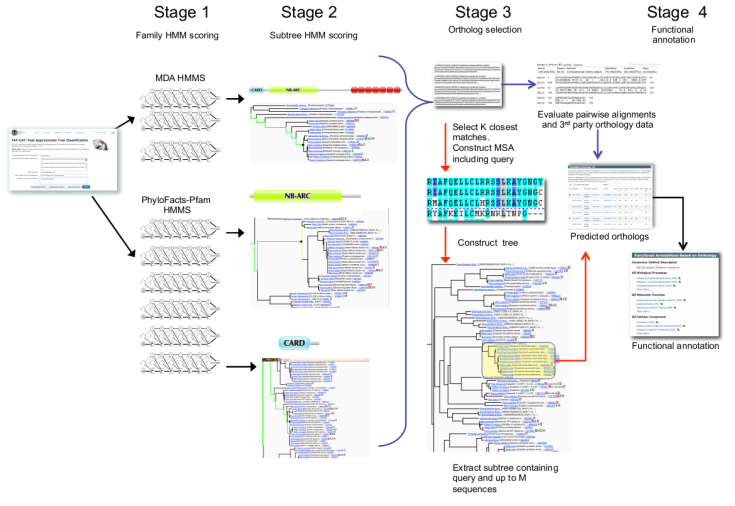
\includegraphics[width=\textwidth]{../Vortrag/figures/fatcat-pipeline.png}
\caption{The \textit{FAT-CAT} workflow pipeline}
\label{fig:fatcat-pipeline}
\end{figure}


\paragraph{How useful is PhyloFacts?}
Within the scope of this report, there are very few aspects that allow to make assumptions about the actual usefulness of SIFTER.

Because these results are likely not significant, this report will list some aspects that seem related to the usefulness without drawing any conclusions.

\begin{itemize}
 \item PhyloFacts is not open-sourced -- in the opinion of the author of this report, it therefore clearly violates the scientific principle of reproducibility. It will be almost impossible to find bugs in both the implementation and the data basis in a complex application like PhyloFacts if the code is not provided to the general public.
 \item Within the 3-day long \textit{FAT-CAT} research for the talk corresponding to this report, the job ID numbers of FAT-CAT ascended monotonically, and increased (on average) by only about 10 per day\footnote{\textit{STRING} had more than 80000 queries per day, averaged over a 7-day period}. It can therefore be assumed that PhyloFacts is not very widely used
 \item \cite{krishnamurthy2006phylofacts} has been cited only 27 times since 2006. While this is more than e.g. \textit{SIMAP} (see \cite{arnold2005simap}) which has been cited 18 times since 2005 and since 2011 been used as STRING data source (see \cite{szklarczyk2011string}), it can be assumed that a widely and publicly adopted tool would be cited more often
 \item The runtime of the tool takes dozends of minutes even for $<300$ AA query sequences
  \item For multiple randomly selected predicted \textit{TrEMBL} sequences\footnote{Example: A1ULI6\_MYCSK}, PhyloFacts did not return any results beside PFam families (said families equivalent to those listed in \textit{UniProt}). Therefore, it did not predict any function for these queries. This aspect might require further research, but raises doubts whether PhyloFacts is useful also for de-novo analyses that don't use known proteins with close relatives in the phylogenetic tree
 \item The SIFTER homepage (\url{http://sifter.berkeley.edu/}) says ``Check back here for a SIFTER server sometime in the next few months!'' since 2006. Although PhyloFacts seems to be updated in several-year intervals, it is neither clear when the underlying database is updated (and, for example, if the parameters change) nor can anyone predict the future of the tool. The ``Encyclopedia'' has completely disappeared since the initial PhyloFacts release.
 \item Conceptually, new sequences require the reconciled tree to incorporate close relatives. For many biologically relevant applications it is possible the tree doesn't contain any such sequence, and it's impossible to reproduce based on a specialized dataset because the application source code is not publically accessible
\end{itemize}

What seems to be useful about PhyloFacts is the attempt of the database to integrate information (especially phylogenetic information) from different sources (e.g. PFAM). If a user has a phylogeny-related question about a query sequence (e.g. \textit{distant clades}), PhyloFacts seems to be able to provide a user-friendly interface (e.g. for biologists that don't want to deal with complex bioinformatics toolsets), as depicted in figure \vref{fig:fatcat-result}.

Additionally, the \textit{FAT-CAT} query supports selectable preset parameters, for example \textit{High recall} and \textit{High precision}.

\begin{figure}[ht!]
\centering
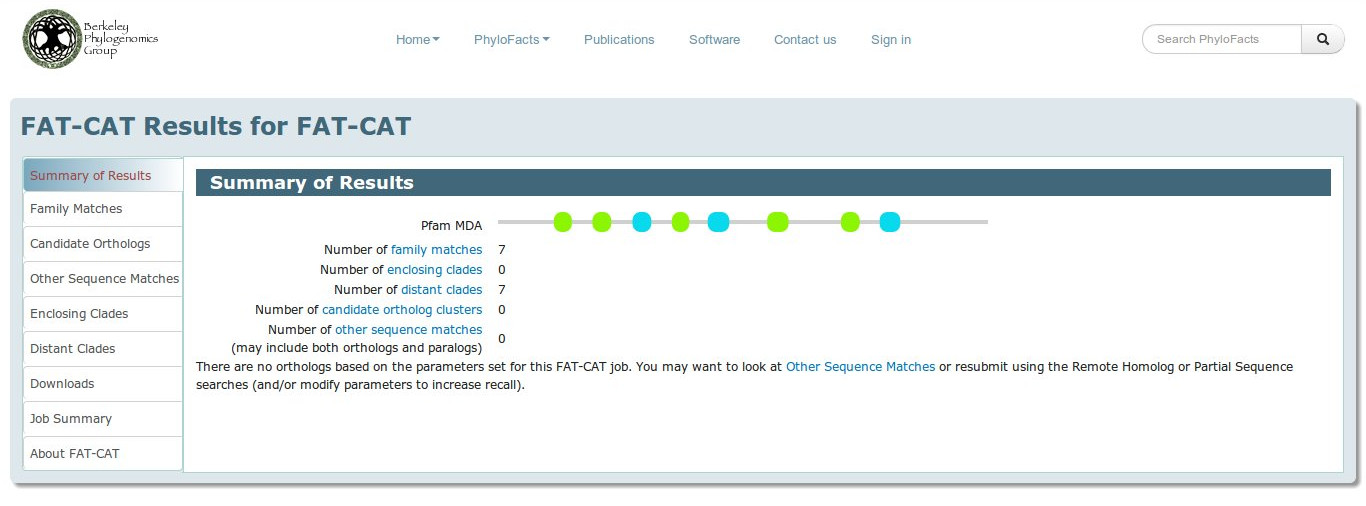
\includegraphics[width=\textwidth]{../Vortrag/figures/fatcat-results.jpg}
\caption{The \textit{FAT-CAT} result page}
\label{fig:fatcat-result}
\end{figure}

\section{Common problems of phylogenomics}\label{sec:problems}

\paragraph{Manual annotation requirement}
As described in section \vref{sec:workflow} the workflow described in \cite{sjolander2004phylogenomic}. While this might improve the quality of the result, essentially it renders the method useless in the context of large-scale analysis as described in section \vref{sec:nonphylo-issues}.

Because of limited availability of expert human resources, phylogenomic analyses with sufficient quality can't be performed on a large scale, even if the computational complexity of the automatable steps would not be an issue.

\paragraph{Huge parameter sets}
The workflow described in \cite{sjolander2004phylogenomic} incorporates several layers of filtering that depend on a large parameterset and even on human factors. It can be assumed that for any real analysis being performed, a large subset of the parameters is chosen suboptimally, because no inherently correct method is known that allows one to choose an optimal parameterset of that size.

In order to achieve optimal results, the parameters would need to be selected for each prediction individually -- however, that is not possible in lack of an absolute reference (representing the biological reality). Almost all algorithms in bioinformatics suffer from similar problems, however in case of phylogenomics the parameterset is -- caused by the large number of steps -- extremely large and contains a large number of known and unknown interdependencies..

Because of the human factor involved in the manual steps, a result may be irreproducible by another researcher, rendering the results subjective.

\paragraph{Parameter sensitivity}
Although a detailed analysis is outside the scope of this report, in \cite{sjolander2004phylogenomic} it is observed that the quality of the results depends on all the filtering passes being present in the workflow. This leads to the conclusion that the non-filter steps are so sensitive to noise that any minimal change in the input data could yield a totally different result.

Because interdependencies in the parameters are largely unknown and the high dimensionality of the parameter space, it is essentially impossible to conclude that any result is not the case of an overyl

This issue gets even more significant in cotext of manual processing: Even if assuming two researchers will select similar options for the same input data, a minor change in the parameters they use could cause the result to change significantly.

\paragraph{Loss of information}
Effectively, the huge parameter sets create a paradox: The phylogenomic method which is intended to augment a prediction by adding new information actually loses a significant amount of information in the filtering passes -- up to an extent where the prediction quality is detrimente. For real predictions (i.e. those lacking an absolute reference), this effect is impossible to detect

\paragraph{Deducing information from itself}\label{p:self-deduction}
Non-phylogenomic methods usually work well for closely-related protein families that will only infrequently express behaviour that yields systematic errors as outlined in section \vref{p:syserrors}. It can be assumed that if a large amount of information is available about a protein, classical methods provide a sufficient prediction quality, rendering phylogenomics useful especially for cases where few information is available.

However, few information being available could hypothetically be detrimental to the phylogenetic tree -- in many cases the information contained in said tree will be derived only from the protein family sequence set itself. However, the same exact sequence set will be used for the classical prediction that will be augmented by phylogenetic information.

Therefore, in an extreme the prediction would actually be augmented with information it already contains, rendering the augmentation useless and (under some circumstances) even decreasing the prediction quality because some aspects of the original prediction are overrated in the final score

It is outside of this report's scope to discuss or assess the effect of this behaviour in general, however it shall be noted that most augmentation methods express a similarly problematic behaviour. The author of this report assumes it is highly problematic to filter out these causality loops, because detailed information about the data sources is not available for any database.

\paragraph{Resolving database issues using phylogenomics}
While \cite{brown2006functional} mentions -- besides the systematic errors outlined in section\vref{p:syserrors} -- the ``propagation of errors in databases'' as a systematic error that can be detrimental to data quality, there seems to be no apparent reason why phylogenomics should be better in resolving those issues than any other method leveraging additional data sources.

To the author of this report, the problems outlined before seem to be too severe to conclude without any doubt that phylogenomics will resolve database issues instead of creating even more ones and making manual result assessment difficult by adding yet another, potentially inaccurate layer of complexity to the prediction.

\section{Conclusion \& Outlook}

Phylogenomics is a method that attempts to augment function prediction by leveraging evolutional information to differentiate orthology and paralogs. Even if a full analysis based on carefully selected test data is outside the scope of this report, the issues described in this report arise doubts whether phylogenomics provides a tool that can be used for real data.

However, issues like the high computational complexity might be partially resolved by advancements in computational hardware or algorithms in the future. \textit{PhyloFacts} provides an example of how a computationally-feasible phylogenomic tool can be predicted, although the quality of the results in contrast to other databases

In practical function prediction, however, it's neccessary to combine any available information and method. Although care has to be taken to ensure the issues of phylogenomics are not detrimental to the result, in many cases other information sources like \textit{context-based prediction} are not sufficient for a significant result.

Therefore, disregarding any practical issues, phylogenomics provide one of many conceptual sources of information, all of which have to be combined to improve in-silico predictions.

\renewcommand\refname{Bibliography}
\bibliographystyle{alphadin}
\bibliography{skript}
\subsection*{Open Data}\label{opendata}
Alle für die Erstellung dieser Ausarbeitung sowie für die Präsentation verwendeten Quelldateien und Rohdaten können dauerhaft unter \url{https://github.com/ulikoehler/Proseminar} abgerufen werden
\end{document}
